\documentclass[12pt]{article}
\usepackage[utf8]{inputenc}
\usepackage[english]{babel}
\usepackage[T1]{fontenc}
\usepackage{amsmath}
\usepackage{amsfonts}
\usepackage{dsfont}
\usepackage{setspace}
\usepackage[dvipsnames]{xcolor}
\usepackage{graphicx}
\usepackage{mathtools}
\usepackage{float}
\usepackage{numprint}
\usepackage{url}
\usepackage{dirtree}
%\usepackage[hidelinks]{hyperref}

\usepackage[Glenn]{fncychap}
\usepackage{enumitem}
\usepackage{multicol}
\pagestyle{plain}
\usepackage{subfig}
\usepackage{siunitx}

% You can set the margine of the text by setting the top, bottom, left and right properties. Also, if using more than one columns, you can change the columnsep property to set the seperation space between two columns.
\usepackage[a4paper,top=30mm,bottom=30mm,columnsep=6mm,left=20mm,right=20mm]{geometry}

% uncommnet and change the following two commands to set seperation line width between coulmns.

% \setlength{\columnsep}{1cm}
% \setlength{\columnseprule}{0.6pt}

%########################## Paper Meta data#########################
% You can change the variables in the following section to set them globally thrghout the whole paper.

% Title of the paper
\newcommand{\papertitle}{Internship notes}
\newcommand{\shorttitle}{}

% Full name of the author(s)
\newcommand{\authorname}{Alexandre CHAUSSARD}

% Module code
\newcommand{\acmodulecode}{01/05/2023}

% Module name
\newcommand{\acmodulename}{}

% Name of the college
\newcommand{\accollegename}{Laboratoire de Probabilité, Statistiques et Modélisation}

% Date
\newcommand{\wrdate}{May 2023}
%########################## Paper Meta data#########################

\usepackage{fancyhdr}

\usepackage{biblatex}
\bibliographystyle{ieeetr}
\addbibresource{library.bib}

\pagestyle{fancy}
\fancyhead{}
\fancyhead[L]{\textsc{\shorttitle}}
\fancyfoot{}
\fancyfoot[R]{\thepage}
\fancyfoot[L]{\acmodulecode\  \textsc{\acmodulename}}
% \fancyfoot[C]{\thepage}
\renewcommand{\headrulewidth}{0.6pt}
\renewcommand{\footrulewidth}{0.6pt}


\title{\papertitle}
\author{\authorname}


\begin{document}

\newcommand{\HRule}{\rule{\linewidth}{0.5mm}} 		
\begin{titlepage}
    \begin{center}
        %\vspace*{1cm}

        \center 
        \begin{figure}[H]
            \centering
            
\includegraphics[width=.5\textwidth]{images/logo_ipp.png}\label{fig:logo_ipp}
        \end{figure}
        
        % Document info
        \textsc{Laboratoire de Probabilité, Statistiques et Modélisation}\\[0.5cm]
        \textsc{\large May 2023}\\[2cm] 
        
        % Course Code
        \HRule \\[1cm]
        { \huge \bfseries Internship report notes}\\[1cm]			
        \HRule \\[.5cm]
        \large

        \vspace*{1cm}
        
        \emph{Master 2 - Data Science} \\[1cm]

        Alexandre CHAUSSARD  \\ [0.5cm]
        
    \end{center}
\end{titlepage}

\newpage
\tableofcontents
\newpage

\section{Introduction}


Given observations of random variables $(X,Y)$, we suppose that there exist another set of random variables $Z$ that we do not observe,
yet that characterize $(X,Y)$ conditionally to $Z$.
$Z$ is then called a latent variable, or a hidden variable. \\

For instance, if we observe the weights of a given population through $X$, and that we aim at inferring their height $Y$, knowing the
sex of each individual through $Z$ could improve our predictions on $Y$.
Hence, assuming that there exist a latent variable to a given model adds structure to the model while improving the explainability,
as $Z$ characterizes the behavior of our dataset.
Typically, clustering methods like KMeans or Gaussian Mixtures Models (GMM) provide a discrete $Z$ given the observations, which are
interesting in the sense that they provide a categorical representation of our data. \\

However, finding such $Z$ given the observations is not straight forward, and not all dataset respond to a latent process, and may be not even a discrete one. \\

During this research internship, we aim at exploring latent models with discrete latent space in order to analyze the microbiota structure.
Our first focus will be on various methods to conceive latent models like Expectation-Maximization and variational models.




\newpage
\section{Variational Auto-Encoders}

\subsection{Framework and optimization objective}

We are interested in another kind of latent models, this time based on variational inference
results to achieve a new kind of deep latent structure: the Variational Auto-Encoder (VAE).
These latent models were introduced in 2013 by Kingma, better described in a more in depth paper in 2019: \cite{kingma2019introduction}

Once again, we assume the observations $X$ to be modelizable by a given distribution
parameterized by $\theta$:

$$
X \sim p_{\theta}(x)
$$

Determining $\theta$ holds to find one $\theta^*$ that would optimize a given objective, generally chosen as the maximum of likelihood. Indeed, if $\theta^* \in arg\max_{\theta} p_{\theta}(x)$, then such $\theta^*$ maximizes the density around the dense areas of the observations, which makes them highly likely to happen under such distribution $p_{\theta^*}$. Hence, the maximum likelihood is a natural criterion:
$$
\theta^* \in arg\max_{\theta} p_{\theta}(x)
$$

However, such modelization does not include a latent structure. As a result, we try to enforce it by rewriting the objective as follows:

$$
p_{\theta}(x) = \int_{\mathcal{Z}} p(x,z) dz 
$$

Using Bayes decomposition, we obtain a computable objective:
$$
p_{\theta}(x,z) = p_{\theta}(z) p_{\theta}(x|z)
$$

Recall that the prior $p_{\theta}(z)$ and the a priori $p_{\theta}(x|z)$ are defined by the framework (ex: Bernoulli prior and Gaussian posterior gives the Gaussian mixture framework). However, the computation of the evidence $p_{\theta}(x)$ is generally intractable in practice, which also leads to a non-tractable posterior distribution: $p_{\theta}(z|x)$. As a result, not being able to compute the evidence leads to not being able to provide a gradient regarding $\theta$, so we can not perform the backpropagation in a deep learning approach.

Note that there exist approximate inference techniques to compute the evidence and the posterior, but these are quite expensive and often yield poor convergence results.

To overcome this issue, we introduce a smart rewriting of the objective using variational inference. Indeed, let $q_{\Phi}(z|x) \approx p_{\theta}(z|x)$ to be learnt over $\Phi$, one can write:
$$
\begin{align}
    \log p_{\theta}(x) &= \mathbb{E}_{q_{\Phi}(z|x)}[\log p_{\theta}(x)] \\
    &= \mathbb{E}_{q_{\Phi}(z|x)}\left[\log \frac{p_{\theta}(x)}{q_{\Phi}(z|x)} \frac{q_{\Phi}(z|x)}{p_{\theta}(z|x)}\right]
    \\
    &= \underbrace{\mathbb{E}_{q_{\Phi}(z|x)} \left[\log \frac{p_{\theta}(x)}{q_{\Phi}(z|x)}\right]}_{ELBO(q_\phi(z|x), p_{\theta}(x,z))} + D_{KL}\left[q_{\Phi}(z|x) \Vert p_{\theta}(z|x)\right]
\end{align}
$$

The first term of that decomposition is generally called the Evidence Lower BOund (ELBO), as it marks a lower bound to the evidence $\log p_{\theta}(x)$ since the KL divergence is a positive quantity:
$$
\log p_{\theta}(x) \ge ELBO(q_\phi(z|x), p_{\theta}(x,z))
$$

$q_{\Phi}(z|x)$ is an approximation of the true posterior $p_{\theta}(z|x)$ that we aim at learning in a family of distributions. For instance, 
$$
q_{\Phi}(.|x) \sim \mathcal{N}(\mu(x), \Sigma(x))
$$ 
would be an approximation of the true posterior by a Gaussian distribution. Notice that the true posterior may very not likely be Gaussian, which creates a first complexity error in our model.

Despite being a lower bound on the true maximum likelihood objective, the ELBO is actually tractable. Indeed, as we continue the computation:
$$
\begin{align}
    ELBO(q_\phi(z|x), p_{\theta}(x,z)) &= \mathbb{E}_{q_{\Phi}(z|x)}[\log p_{\theta}(x,z)] - \mathbb{E}_{q_{\Phi}(z|x)}[\log q_{\Phi}(z|x)] \\
    &= 
\mathbb{E}_{q_{\Phi}(z|x)}[\log p_{\theta}(x|z)] - D_{KL}[\log q_{\Phi}(z|x) \Vert p_{\theta}(z)] \\\end{align}
$$

Another remarkable fact, is that when maximizing the ELBO, we are actually minimizing the KL divergence between the estimated and the true posterior. Hence, one can define the ELBO as a suboptimal objective to our problem that we get to maximize to obtain $(\Phi^*, \theta^*)$, the parameters of our model.

\subsection{Reparameterization trick}

Even though the gradient of the ELBO is well defined for $\theta$, it is not possible to compute it relatively to $\Phi$ it requires samples from the approximation to the posterior $q_{\Phi}(z|x)$ to compute $\mathbb{E}_{q_{\Phi}(z|x)}[\log p_{\theta}(x|z)]$. 

Since, sampling is not a differentiable operation, we make use of the change of variable formula, so that for a bijective transformation $z = \phi_x(\epsilon)$, we get:
$$
p(z) = p(\epsilon) \det \left| \frac{\partial \epsilon}{\partial z}\right|
$$

Hence, if we take $\epsilon$ a random variable of density $p(\epsilon)$ that does not depend on $\theta$, $\Phi$ nor $x$, so that $z = \phi_x(\epsilon)$, for any $L_1$ function $f$,
$$
\mathbb{E}_{q_{\Phi}(z|x)}[f(z)] = \mathbb{E}_{p(\epsilon)}[f(z)]
$$

As a result, the samples are not obtained through $q_{\Phi}$ anymore but through $p(\epsilon)$, so that can safely perform derivation of the ELBO relatively to $\Phi$ and backpropagate our gradient through the network.

\subsection{Architecture}

The vanilla architecture of the VAE is described by the following illustration:

[ILLUSTRATION VAE]

The first part is generally called the encoder, as it turns a sample $x$ into its latent representation $z$ by modelizing the posterior $q_{\Phi}(z|x)$. The second part is then called the decoder, as it throws a latent representation in the sample space. The latest can even serve as a generative architecture, as one can sample from the latent space through $q_{\Phi}(z|x)$, and decode it to obtain a new sample.

As we can see more clearly in that illustration, we can see that $\Phi$ and $\theta$ are trained jointly through the ELBO, both serving for one part of the VAE at a time.

The training procedure is straightforward: the entry is a sample $x$ and the output objective is the same sample $x$. We aim at train the VAE for learning the data space and its latent representation by learning how to reconstruct the samples through it.




\newpage
\section{VQ-VAE}

\subsection{Quick overview}

Introduced in \cite{vq_vae_paper}, VQ-VAE architecture provides a framework to compute
discrete posterior distributions $q_{\Phi}(z|x)$.
To compare that model with the VAE, we start by introducing the architecture of the model for which an illustration is given below:

\begin{figure}[H]
    \centering
    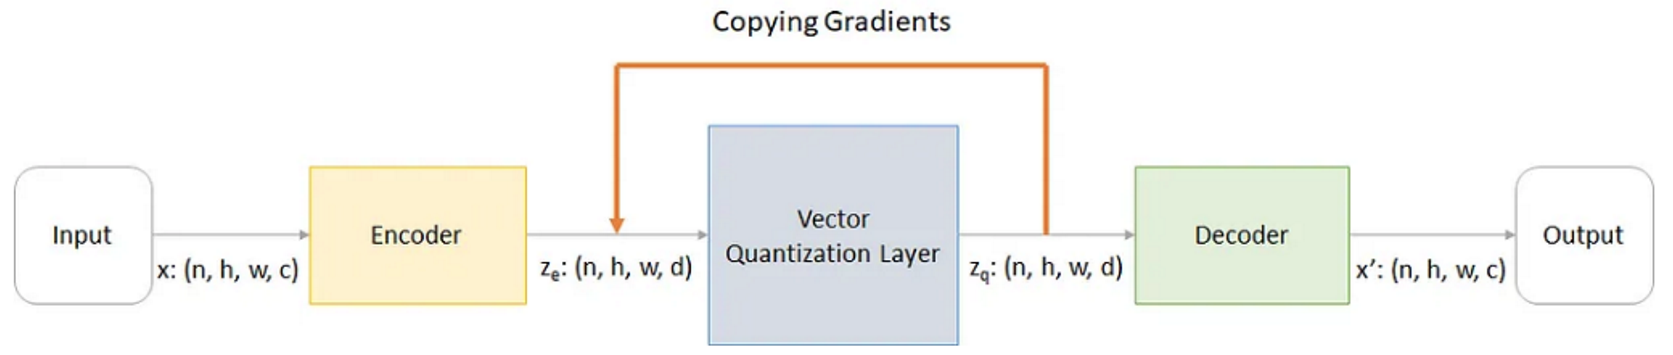
\includegraphics[width=.9\textwidth]{images/vq_vae_architecture}
    \caption{VQ-VAE architecture (source: Medium)}
    \label{fig:vq_vae_architecture}
\end{figure}

As we can see on figure \ref{fig:vq_vae_architecture}, the major difference with the vanilla VAE architecture
lies in the vector quantization step which enables to project the output of the encoder denoted by $z_e(x)$
onto a discrete embedding dictionary $(e_1, \dots, e_K)$ by a simple distance argument:
$$
k = arg\min_{j} \Vert z_q(x) - e_j \Vert_2, \quad z_q(x) = e_k
$$

The projection of $z_e(x)$ on that discrete dictionary is denoted by $z_q(x)$, and serves as the input of the decoder.
For further visual representation of the vector quantization layer, an illustration is given below.

\begin{figure}[H]
    \centering
    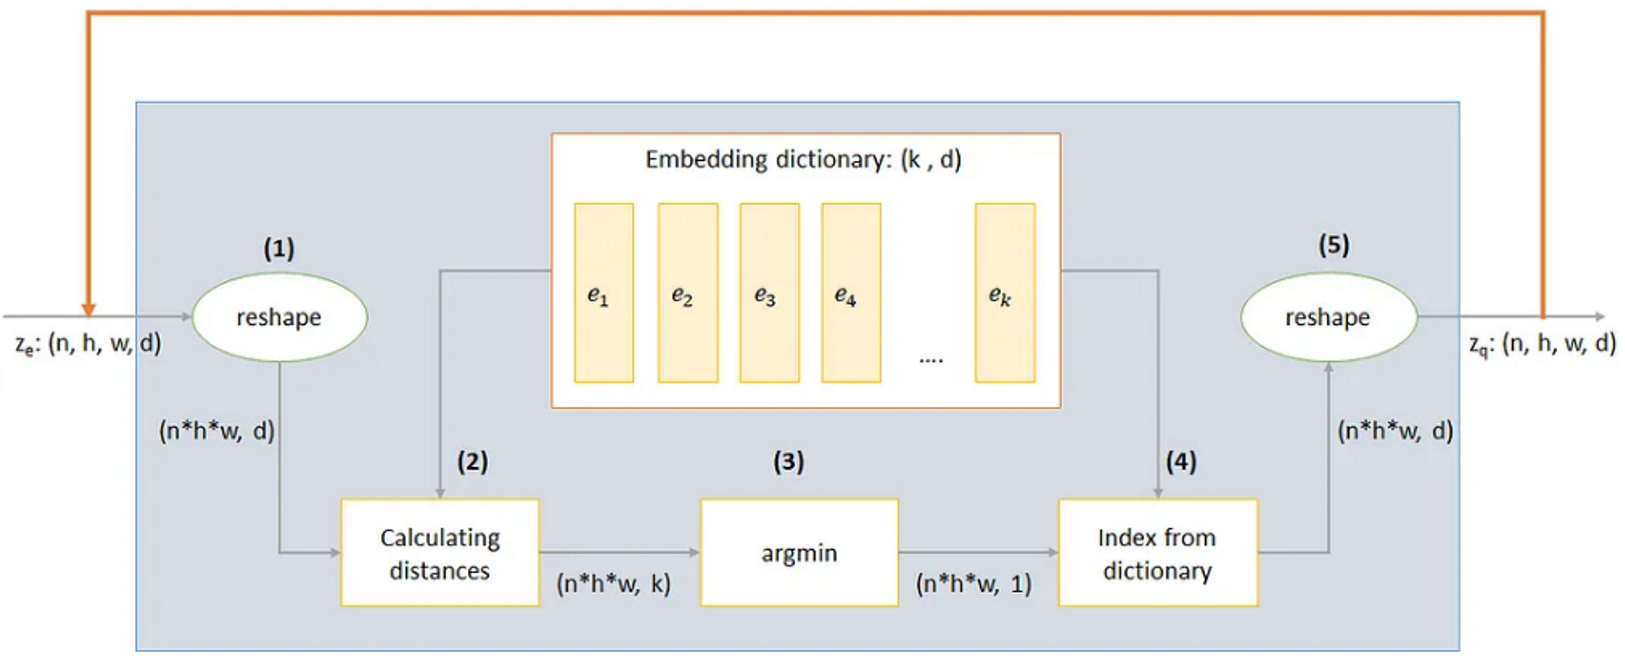
\includegraphics[width=.7\textwidth]{images/vq_vae_quantization}
    \caption{Architecture of the VQ-VAE: quantization layer (source: Medium)}
    \label{fig:vq_vae_quantization}
\end{figure}

Looking at the previous figures, we can grasp the challenge of backpropagation in such model with discrete prior and posterior.
In the next section, we enter in the mathematical definition of the objective and how to train this architecture.

\subsection{Framework and optimization objective}

Contrary to the vanilla VAE, we have the following categorical distributions assumption:
\begin{itemize}
    \item The prior $p_{\theta}(z)$ is categorical.
          In the original paper, it is taken as uniform supported in $\{1, \dots, K\}$ during the training.
          When the training is over, it is fit to an autoregressive distribution through a PixelCNN (see \cite{pixel_cnn_paper}).
          It is left as an exploration research field to be able to learn the prior while training the model.
    \item The posterior $q_{\Phi}(z|x)$ is categorical and set to the following:
          $$
          q_{\Phi}(k|x) = \mathds{1}_{\{k = arg\min_{j} \Vert z_q(x) - e_j \Vert_2\}}
          $$
\end{itemize}

This modelization of the posterior enables to obtain a discrete latent space, but it does not allow to differentiate regarding $\Phi$.
As a result, the authors suggest two possible strategies:
\begin{itemize}
    \item \textit{Straight-through}: propagate the gradient through the discrete part (vector quantization layer) without changing it.
          The intuition is that the gradient propagated from the encoder contains sufficient information to update the encoder accordingly, but this is just intuition.
    \item \textit{Subgradient}: compute the subgradient of the quantization layer (unexplored yet)
\end{itemize}

The optimization objective of the VQ-VAE is based on the ELBO, that one can compute as follow:
$$
\begin{align}
    ELBO(q_{\Phi}(z|x), p_{\theta}(z|x)) &= \mathbb{E}_{q_{\Phi}(z|x)}[\log p_{\theta}(x,z)] - \mathbb{E}_{q_{\Phi}(z|x)}[\log q_{\Phi}(z|x)] \\
    &= \mathbb{E}_{q_{\Phi}(z|x)}[\log p_{\theta}(x|z)] - D_{KL}[q_{\Phi}(z|X) \Vert p_{\theta}(z)]
\end{align}
$$

Notice then that:
\begin{itemize}
    \item Since $q_{\Phi}(k|x) = \mathds{1}_{\{k = arg\min_{j} \Vert z_q(x) - e_j \Vert_2\}}$, we have:
          $$
          \begin{align}
              \mathbb{E}_{q_{\Phi}(z|x)}[\log p_{\theta}(x|z)] = \log p_{\theta}(x|z_q(x))
          \end{align}
          $$
    \item Since $Z \sim \mathbb{U}(\{1, ..., K\})$, $\mathbb{P}(Z=k) = \frac{1}{K}$.
          Also, notice that $q_{\Phi}(z_q(x)|x) = 1$ by definition of $q_{\Phi}(z|x)$ and $z_q(x)$.
          Combining those results, we obtain:
          $$
          \begin{align}
              D_{KL}[q_{\Phi}(z|x) \Vert p_{\theta}(z)] &= \mathbb{E}_{q_{\Phi}(z|x)}\left[\log \frac{q_{\Phi}(z|x)}{p_{\theta}(z)} \right] \\
              &= \log \frac{q_{\Phi}(z_q(x)|x)}{p_{\theta}(z_q(x))} \\
              &= \log K
          \end{align}
          $$
          Therefore, this KL divergence does not impact the optimization objective as it does not depend on ($\theta$, $\Phi$).
\end{itemize}

Computing the previous quantities, we would obtain the following suboptimal objective for the VQ-VAE:
$$
ELBO(\Phi, \theta) = log p_{\theta}(x|z_q(x))
$$

However, such objective does not enable to learn the dictionary since we use a straight-through approach over the quantization layer.
To update the dictionary, the authors suggest to add the following term to the loss:
$$
\Vert sg[z_e(x)] - e \Vert_2^2
$$
Where $sg$ denotes the stop-gradient operator, meaning we do not consider any gradient after the given operation.
\medskip

Finally, to prevent embedding space over expansion, the authors suggest the addition of a commitment loss parameterized by $\beta > 0$:
$$
\beta \Vert z_e(x) - sg[e] \Vert_2^2
$$
Indeed, the embedding space was unconstrained so far, so its dimension could grow arbitrarily.
Intuitively, adding that term forces the model to commit to a given embedding.
\medskip

Overall, we obtain this final objective to maximize:
$$
\mathcal{L}(\theta, \Phi) = \log p_{\theta}(x|z_q(x)) + \Vert sg[z_e(x)] - e \Vert_2^2 + \beta \Vert z_e(x) - sg[e] \Vert_2^2
$$

\subsection{Discussion over some limiting aspects}

Even though the previous objective seems natural, we only rigorously justified the first term thanks to the ELBO.
Indeed, the dictionary update loss as well as the commitment loss keep dropping out from nowhere, while they seem necessary to ensure the training of our model.
\medskip

Furthermore, we did not really deal with the non differentiability of the vector quantization loss, and the straight-through estimator
can definitely be criticized about what information it actually provides to the encoder to update appropriately.
\medskip

Finally, the usage of the PixelCNN after the training seems very unnatural, and could significantly boost the model as the PixelCNN did show amazing performances so far.
\newpage
\section{PixelCNN}

\subsection{Overview}

Introducing the VQ-VAE, we have seen that an under-table tool that was being used is the Pixel CNN,
first introduced in \cite{pixel_cnn_paper}.
In the context of the VQ-VAE, it plays a major role after training by learning the prior $p(z)$, that was set
to a discrete uniform previously.
This makes a drastic difference with the VAE, as we are not setting the prior ourselves as it's being learnt and modeled by the PixelCNN in this process.
\medskip

Indeed, the PixelRNN/PixelCNN architectures are sequential deep neural networks that aims at modeling the distribution of a data space
in an autoregressive fashion.
Their main characteristic is that they take advantage of the structure of an image to learn the data space distribution.
\begin{itemize}
    \item \textit{PixelRNN}: Bi-directional recurrent networks with variable smart directions are used to model the spatial dependencies between pixels.
    (3 architectures are presented in the original paper, but our focus will be on the PixelCNN here).

    \item \textit{PixelCNN}: the dependencies between the pixels is modeled through stacking of masked convolution layers (it's faster since the receptive field is bounded by the size of the convolution), no pooling layer is used.
    The masking ensures that we keep an autoregressive estimation of a new pixel, without seeing the future pixels.
\end{itemize}

The following figure illustrates the masked convolution technique.
\begin{figure}[H]
    \center
    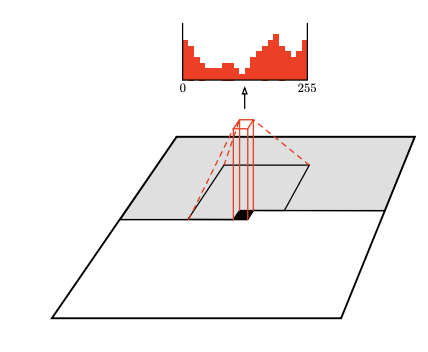
\includegraphics[scale=0.9]{images/masked_convolution_pixel_cnn}
    \caption{Masked convolution on an image (largest square), the big square represents the receptive field of the black pixel, the white area is masked}
    \label{fig:masked_convolution_pixel_cnn}
\end{figure}

Hence, given $x$ an image represented by its pixels $x = (x_1, \dots, x_n)$, as usual for these distribution modeling problems, we aim at finding $\theta^* = arg\max_{\theta} p_{\theta}(x)$ in a family of distributions parameterized by $\theta$: the maximum of likelihood.
Contrary to the usual independent framework, we consider a local dependency between pixels given by the receptive field of our convolution.
This local dependency is limited to the already seen pixels only as well, thanks to the masked convolution.
\medskip

Furthermore, rather than using continuous outputs, these architecture use a softmax layer to determine the pixel of a given generation,
leading to a discrete prior rather than a continuous one, which is required for the VQ-VAE for instance.
As a result, the distribution of a pixel conditionally to the ones in its receptive field is given by a multinomial in $\{0, \dots, 256\}$.
\medskip

\subsection{Usage in the VQ-VAE}

Once we have trained the VQ-VAE, the original paper states that we can replace the uniform prior on $p(z)$ by a PixelCNN to model the prior.
To perform the training of the PixelCNN, we turn the samples $x$ in their latent representations $z$, and train the PixelCNN over the latent representations $z$.
This way, we have created dependency between the $z$ in the latent feature mapping, and we obtain a prior over their distribution modeled by the PixelCNN.



\newpage
\section{Bibliography}
% \pagebreak
\nocite{*}
\printbibliography

\end{document}